% CS F407 final report, Team 22 (Saul Goodman). Style follows the submitted proposal (docs/proposal/AIPP_Team22_SaulGoodman.pdf).
% Build: python report/build_report.py   (needs tectonic). Every result number is a macro from generated/numbers.tex or a generated table.
\documentclass[11pt,a4paper]{article}
\usepackage[margin=2.2cm,top=2.4cm,bottom=2.2cm]{geometry}
\usepackage{fontspec}
\setmainfont{texgyrepagella}[Extension=.otf,UprightFont=*-regular,BoldFont=*-bold,ItalicFont=*-italic,BoldItalicFont=*-bolditalic]
\setsansfont{texgyreheros}[Extension=.otf,UprightFont=*-regular,BoldFont=*-bold,ItalicFont=*-italic,BoldItalicFont=*-bolditalic]
\setmonofont{texgyrecursor}[Extension=.otf,UprightFont=*-regular,BoldFont=*-bold,ItalicFont=*-italic,BoldItalicFont=*-bolditalic,Scale=0.88]
\usepackage{amsmath,amssymb,unicode-math}
\setmathfont{texgyrepagella-math.otf}
\usepackage{booktabs,tabularx,graphicx,xcolor,microtype,enumitem,caption,longtable,array}
\usepackage{tikz}
\usetikzlibrary{positioning,arrows.meta,shapes.geometric,fit,calc}
\usepackage[hidelinks]{hyperref}
\usepackage{fancyhdr}
\usepackage{titlesec}
\definecolor{navy}{HTML}{1B2A49}
\definecolor{accent}{HTML}{2F6DB5}
\definecolor{todo}{HTML}{B3261E}
\titleformat{\section}{\large\bfseries\color{navy}}{\thesection.}{0.6em}{}
\titleformat{\subsection}{\normalsize\bfseries\color{navy}}{\thesubsection}{0.6em}{}
\setlist{nosep,leftmargin=1.4em}
\captionsetup{font=small,labelfont=bf}
\setlength{\emergencystretch}{3em}\setlength{\parindent}{0pt}\setlength{\parskip}{0.55em}
\pagestyle{fancy}\fancyhf{}
\lhead{\small\itshape CS F407 Artificial Intelligence, Final Report}\rhead{\small\itshape Team 22, Saul Goodman}\cfoot{\thepage}
\renewcommand{\headrulewidth}{0.4pt}
\newcommand{\todo}[1]{\textcolor{todo}{\textbf{[#1]}}}
\newcommand{\file}[1]{\texttt{#1}}
% generated by report/build_report.py: do not edit
\newcommand{\NCases}{10}
\newcommand{\NMove}{4}
\newcommand{\NEvidence}{6}
\newcommand{\MSeeds}{8}
\newcommand{\NLawyers}{3}
\newcommand{\NPartly}{1}
\newcommand{\BootSeeds}{200}
\newcommand{\BootResamples}{200}
\newcommand{\BootWorstPlain}{87.0\%}
\newcommand{\BootWorstPlainCase}{The Broken Bike}
\newcommand{\BootBelowPlain}{0}
\newcommand{\BootBelowSurprises}{1}
\newcommand{\BootWorstSurprises}{60.5\%}
\newcommand{\BootWorstSurprisesCase}{The Dug-Up Garden}
\newcommand{\BootWorstAny}{60.5\%}
\newcommand{\BootWorstAnyCase}{The Dug-Up Garden}
\newcommand{\BootWorstAnyMode}{surprises on}
\newcommand{\NSearches}{6}
\newcommand{\NBeaten}{4}
\newcommand{\BestGain}{1.59}
\newcommand{\BestCase}{Helix Dynamics Trade-Secret Exfiltration}
\newcommand{\ClassicCorners}{360}
\newcommand{\ClassicFoundTotal}{0}
\newcommand{\MatchingPennies}{16}
\newcommand{\SearchTried}{395}
\newcommand{\SearchLookedDilemma}{41}
\newcommand{\SearchLookedStag}{6}
\newcommand{\SearchKept}{0}
\newcommand{\ClassicSeeds}{200}
\newcommand{\EffSeeds}{200}
\newcommand{\TheoremHolds}{20}
\newcommand{\TheoremTotal}{20}
\newcommand{\TreeSolved}{17}
\newcommand{\TreeTotal}{18}
\newcommand{\LookSeeds}{40}
\newcommand{\LookBeats}{1}
\newcommand{\LookBeatsCase}{AV-7 Crosswalk Collision}
\newcommand{\SensVariations}{14}
\newcommand{\SensSeeds}{16}
\newcommand{\SensRobust}{3}
\newcommand{\SensFragile}{7}
\newcommand{\NCommits}{168}
\newcommand{\NAuthors}{10}
\newcommand{\NCommitDays}{40}
\newcommand{\FirstCommit}{2026-09-27}
\newcommand{\LastCommit}{2026-11-17}
\newcommand{\TrialMedianMs}{2.7}
\newcommand{\TrialMaxMs}{23.2}
\newcommand{\TimedTrials}{160}
\newcommand{\ReplaySame}{160}
\newcommand{\ReplayTotal}{160}
\newcommand{\ReplayChain}{160}
\newcommand{\StressTrials}{2500}
\newcommand{\StressCrashes}{0}
\newcommand{\StressInvariant}{0}
\newcommand{\StressReplays}{2500}
\newcommand{\StressMeanMs}{1.644}
\newcommand{\CourseCommits}{82}
\newcommand{\CourseAuthors}{8}
\newcommand{\CourseFirst}{2026-10-02}
\newcommand{\CourseLast}{2026-11-11}
\newcommand{\CourseDays}{33}
\newcommand{\CourseMinPerDay}{2}
\newcommand{\CourseMaxPerDay}{3}
\newcommand{\CourseSame}{23}
\newcommand{\CourseDiffer}{3}
\newcommand{\CourseCore}{26}
\newcommand{\LumpDate}{2026-09-27}
\newcommand{\CourseAditya}{8}
\newcommand{\CourseDivvij}{10}
\newcommand{\CourseLakshya}{1}
\newcommand{\CourseMofasser}{8}
\newcommand{\CoursePramit}{14}
\newcommand{\CourseRakshit}{16}
\newcommand{\CourseBinary}{19}
\newcommand{\CourseRohan}{6}
\newcommand{\CourseFirstAgents}{2026-10-17}
\newcommand{\CourseFirstCases}{2026-10-12}
\newcommand{\CourseFirstContracts}{2026-10-12}
\newcommand{\CourseFirstEngine}{2026-10-18}
\newcommand{\CourseFirstGametheory}{2026-10-19}
\newcommand{\CourseFirstJudge}{2026-10-15}
\newcommand{\CourseFirstProcedure}{2026-10-13}
\newcommand{\DefenseOnlySpent}{0.5}
\newcommand{\EOneDigests}{37}
\newcommand{\EOneTrials}{160}
\newcommand{\EOneFlipped}{2}
\newcommand{\CommitsPramit}{72}
\newcommand{\FirstPramit}{2026-10-17}
\newcommand{\LastPramit}{2026-11-17}
\newcommand{\ClaudePramit}{0}
\newcommand{\AllCommitsPramit}{72}
\newcommand{\CommitsBinarycoder}{31}
\newcommand{\FirstBinarycoder}{2026-10-02}
\newcommand{\LastBinarycoder}{2026-11-17}
\newcommand{\ClaudeBinarycoder}{0}
\newcommand{\AllCommitsBinarycoder}{31}
\newcommand{\CommitsRakshitGoel}{16}
\newcommand{\FirstRakshitGoel}{2026-10-22}
\newcommand{\LastRakshitGoel}{2026-11-10}
\newcommand{\ClaudeRakshitGoel}{0}
\newcommand{\AllCommitsRakshitGoel}{16}
\newcommand{\CommitsPramitKH}{14}
\newcommand{\FirstPramitKH}{2026-10-11}
\newcommand{\LastPramitKH}{2026-11-08}
\newcommand{\ClaudePramitKH}{0}
\newcommand{\AllCommitsPramitKH}{14}
\newcommand{\CommitsDivvij}{11}
\newcommand{\FirstDivvij}{2026-09-30}
\newcommand{\LastDivvij}{2026-11-11}
\newcommand{\ClaudeDivvij}{0}
\newcommand{\AllCommitsDivvij}{11}
\newcommand{\CommitsMofasserArafat}{8}
\newcommand{\FirstMofasserArafat}{2026-10-17}
\newcommand{\LastMofasserArafat}{2026-11-06}
\newcommand{\ClaudeMofasserArafat}{0}
\newcommand{\AllCommitsMofasserArafat}{8}
\newcommand{\CommitsAditya}{8}
\newcommand{\FirstAditya}{2026-10-11}
\newcommand{\LastAditya}{2026-11-05}
\newcommand{\ClaudeAditya}{0}
\newcommand{\AllCommitsAditya}{8}
\newcommand{\Commitsrohanp}{6}
\newcommand{\Firstrohanp}{2026-10-19}
\newcommand{\Lastrohanp}{2026-11-09}
\newcommand{\Clauderohanp}{0}
\newcommand{\AllCommitsrohanp}{6}
\newcommand{\CommitsLakshyaSachdeva}{1}
\newcommand{\FirstLakshyaSachdeva}{2026-10-02}
\newcommand{\LastLakshyaSachdeva}{2026-10-02}
\newcommand{\ClaudeLakshyaSachdeva}{0}
\newcommand{\AllCommitsLakshyaSachdeva}{1}
\newcommand{\CommitsSavage}{1}
\newcommand{\FirstSavage}{2026-09-27}
\newcommand{\LastSavage}{2026-09-27}
\newcommand{\ClaudeSavage}{0}
\newcommand{\AllCommitsSavage}{1}
\newcommand{\ClaudeTotal}{0}
\newcommand{\AllCommitsTotal}{168}
\newcommand{\FlagshipEvidence}{Aurora Protocol Flash-Loan Exploit}
\newcommand{\OracleBudget}{60}
\newcommand{\ReviewTotal}{70}
\newcommand{\ReviewFixed}{34}
\newcommand{\ReviewDeferred}{35}
\newcommand{\ReviewRejected}{1}
\newcommand{\ReviewPZeroFixed}{1}
\newcommand{\ReviewPOneFound}{20}
\newcommand{\ReviewPOneFixed}{17}
\newcommand{\BootOldSeeds}{100}
\newcommand{\BootOldBelow}{2}
\newcommand{\BootOldWorst}{35.0\%}
\newcommand{\BootOldWorstCase}{The Broken Bike}
\newcommand{\BootOldSecondCase}{AV-7 Crosswalk Collision}
\newcommand{\BootOldSecond}{53.5\%}
\newcommand{\SensPriorChanges}{6}
\newcommand{\TestsAnalysis}{73}
\newcommand{\TestsFailedAnalysis}{0}
\newcommand{\TestsCorrectness}{106}
\newcommand{\TestsFailedCorrectness}{0}
\newcommand{\TestsLiveDemo}{215}
\newcommand{\TestsFailedLiveDemo}{0}
\newcommand{\TestsRobustness}{467}
\newcommand{\TestsFailedRobustness}{0}


\begin{document}
\thispagestyle{empty}
\begin{center}
\vspace*{0.5cm}
{\large\bfseries A REPORT}\\[0.5em] {\small\bfseries ON}\\[1.2em]
{\Large\bfseries STRATEGIC AI AGENTS\\IN A SIMULATED COURTROOM}\\[1.6em]
{\small\bfseries BY}\\[0.8em]
{\small\begin{tabularx}{\textwidth}{@{}p{3.6cm}p{2.6cm}X@{}}
\toprule
\textbf{Name of the students} & \textbf{ID No(s).} & \textbf{Discipline(s)}\\
\midrule
Divvij Yogesh Chichra & 2024AAPS0298H & B.E. Electronics and Communication\\
Lakshya Sachdeva & 2024A8PS0468H & B.E. Electronics and Instrumentation\\
Mofasser Arafat Midda & 2023B1A80965H & M.Sc. Biological Sciences and B.E. Electronics and Instrumentation\\
Pramit Khandelwal & 2024A3PS0443H & B.E. Electrical and Electronics\\
Rakshit Goel & 2023A3PS0373H & B.E. Electrical and Electronics\\
Aditya Singh & 2024A8PS0491H & B.E. Electronics and Instrumentation\\
Rohan Baban Pagire & 2024A7PS1160H & B.E. Computer Science\\
\bottomrule
\end{tabularx}}\\[2em]
{\bfseries Prepared in partial fulfillment of the}\\[0.8em]
{\Large\bfseries Course CS F407: Artificial Intelligence}\\[0.5em]
{\small\bfseries Final Report, Team 22 (Saul Goodman)}\\[0.3em]
{\small\bfseries Track: Demo \quad Topic: Agents \& Game Theory}\\[1.2em]

\includegraphics[width=3.6cm]{figures/bits_logo.png}\\[1.2em]
{\bfseries BIRLA INSTITUTE OF TECHNOLOGY \& SCIENCE, PILANI}\\[0.3em]
{\small\bfseries Hyderabad Campus}\\[0.8em]
{\bfseries November 2026}
\end{center}
\newpage

\begin{center}
{\large\scshape CS F407 Artificial Intelligence\quad Final Report\quad Overview}\\[0.8em]
{\LARGE\bfseries Strategic AI Agents in a Simulated Courtroom}\\[0.3em]
{\itshape Evidence, objections and limited budgets, played as a game between two rational agents}
\end{center}

\begin{tabularx}{\textwidth}{@{}lX@{}}
\textbf{Project name} & Strategic AI Agents in a Simulated Courtroom\\
\textbf{Team} & Team 22, Saul Goodman (7 members)\\
\textbf{Course} & CS F407 Artificial Intelligence, BITS Pilani, Hyderabad Campus\\
\textbf{Track} & Demo\\
\textbf{Topic area} & Agents \& Game Theory (the rule-based judge also draws on Knowledge Representation \& Reasoning)\\
\textbf{GitHub repository} & \url{https://github.com/AI-Projects-S1-26-27/T22_SAUL_GOODMAN}\\
\textbf{Live demo} & \texttt{python -m courtroom serve}, then \texttt{http://127.0.0.1:8000}; a static copy with recorded trials is hosted (see \file{README.md})\\
\end{tabularx}

\paragraph{Abstract.} We built a multi-agent courtroom as a small formal game: two lawyer agents with limited budgets present, object to and challenge exhibits that carry hidden defects, and a deterministic rulebook judge with exact arithmetic rules on every objection and decides the verdict. On top of the simulator, a game-theory layer estimates payoff tables over \BootSeeds{} common seeds, solves them for Nash equilibria in exact rationals, and tests how stable each conclusion is under resampling, under changes to the rulebook's constants and against a search for better lawyers. Across the \NCases{} cases of the library, the lawyers' strategies move the verdict in only \NMove{} cases; the other \NEvidence{} are decided by the evidence alone. We report what held, what did not, and what we could not find.

\tableofcontents
\newpage

\section{Introduction}\label{sec:intro}

\subsection{Problem and project question}
A trial is a small resource-allocation game. Each side has a limited budget and has to decide what goes on the record, what to challenge and when to stop. A doubtful exhibit can help, but if the other side objects on the right ground it is thrown out and the presenter is penalised. Objecting to everything is not free either: it uses budget, and an overruled objection is itself sanctioned. Neither side can see which of the other's exhibits really carry a defect, and neither knows what the opponent will do next. The same structure, costly challenges against hidden flaws under a budget, appears in audits, peer review and security inspections, so the trial is a familiar instance of it.

\begin{quote}\itshape
Against a fixed and fully transparent judge, how do budgets, penalties and noisy perception decide whether an aggressive or a conservative strategy wins, and for which cases does the game have a dominant strategy rather than a mixed equilibrium?
\end{quote}

This is the question of our proposal. The feedback on the earlier topic submission set three requirements: a deterministic, well-defined verdict rule; robustness to weak, missing or contradictory evidence; and synthetic cases only. Section~\ref{sec:method} shows how the design meets the first, Section~\ref{sec:results} the second, and every case, person and organisation in the library is invented.

\subsection{Contribution}
We claim no new algorithm and no accuracy on real cases. The contribution is an inspectable formal game and a set of measurements on it that anyone can reproduce:
\begin{itemize}
\item a \emph{simulator}: typed case files, a phase state machine with an action validator, four lawyer styles, an exact rulebook judge, and a hash-chained event log, so that the same case, styles and seed give the same trial every time;
\item a \emph{game-theory layer}: payoff tables from simulation, exact Nash equilibria, bootstrap stability, sensitivity to the rulebook's constants, a search for better lawyers, and the lecture concepts (classic games, Pareto efficiency, security values, minimax and alpha-beta) computed on our own games;
\item a \emph{demo}: a web application that plays any recorded trial in a 3D courtroom with pre-recorded voices, runs fresh trials on the local server, lets an examiner edit or write a case, and a ``strategy lab'' page that walks through the analysis.
\end{itemize}

\subsection{What was delivered}
The library has \NCases{} synthetic cases: three flagship cases (a cyber-espionage prosecution, an autonomous-vehicle liability suit and a DeFi exploit dispute), three everyday cases, and four edge fixtures. The 16 pairings of the four styles on each case, at seed~0, give \ReplayTotal{} recorded trials, whose digests are pinned by a test. All numbers in this report are generated from the stored result files under \file{results/} by scripts, so a reader can regenerate any of them (Section~\ref{sec:repro}). Where the project differs from the proposal, Section~\ref{sec:deviations} says so.

\subsection{Roadmap}
Section~\ref{sec:related} places the work among related systems. Section~\ref{sec:method} describes the method. Section~\ref{sec:results} goes through the proposal's evaluation plan row by row and reports the analysis results. Section~\ref{sec:discussion} discusses limits and reflects on how the work was done. Sections~\ref{sec:contrib} and~\ref{sec:ai} give the individual contributions and the AI usage.

\section{Background and related work}\label{sec:related}

\subsection{Course concepts used}
\begin{center}\small
\begin{tabularx}{\textwidth}{@{}p{3.4cm}Xl@{}}
\toprule
\textbf{Concept} & \textbf{How it is used here} & \textbf{Package}\\
\midrule
Rational agents, expected utility \cite{russell} & Each lawyer maximises $U = 10\cdot\mathbf 1[\text{win}] - 0.3\cdot\text{spent} - 1.0\cdot\text{sanctions}$ (constants in \file{engine/utility.py} and \file{agents/base.py}). The payoff is not zero-sum, so the game is general-sum. & \file{agents/}\\
Decision under uncertainty, Bayes' rule \cite{russell} & A noisy red-flag signal about each exhibit is turned into a posterior probability that a defect exists; the Smart style also tracks the opponent's objection rate with a Beta posterior. & \file{agents/}\\
Game formulation: states, actions, transitions, terminal test \cite{russell} & The trial is a finite state machine with typed legal actions, turn caps and guaranteed termination. & \file{procedure/}\\
Normal-form games, Nash equilibrium, empirical game analysis \cite{shoham,nash,porter,wellman} & Payoff bimatrices over styles estimated from simulation; pure equilibria by scanning, mixed ones by support enumeration in exact rationals, iterated dominance elimination and an independent best-response check. & \file{gametheory/}\\
Evolutionary dynamics \cite{taylor} & Replicator dynamics on the payoff tables (\file{gametheory/dynamics.py}). & \file{gametheory/}\\
Incentive (parameter) design \cite{shoham} & Costs, sanctions and budgets are game parameters; a sweep moves them and re-solves (Section~\ref{sec:results}). No incentive-compatibility claim is made. & \file{judge/}\\
Rule-based reasoning (KR\&R) & The judge is a forward-applied rule system: every ruling names a rule ID, so each score change and verdict can be traced. & \file{judge/}\\
Minimax, alpha-beta, game trees \cite{russell} & The trial as a tree, solved exactly on an open-file relaxation, with pruning measured. & \file{gametheory/search.py}\\
\bottomrule
\end{tabularx}
\end{center}

\subsection{Related work}
We read the abstract page of each paper named in this subsection and describe only what that page states; Wellman's and McMahan et al.'s papers were not retrieved and are cited by title only.

\paragraph{Courtroom simulation with language models.} AgentsCourt \cite{agentscourt} proposes a multi-agent framework that mirrors a court trial, with a debate simulation, legal-resource retrieval and decision refinement, to simulate a judge's decision. It introduces a benchmark of 420 Chinese judgment documents. AgentCourt \cite{agentcourt}, a different paper, simulates a court in which lawyer agents improve through adversarial interaction; its abstract reports evaluation on a new benchmark, CourtBench, and on 1,000 simulated civil cases. The Strategic Courtroom Framework \cite{siedler} has prosecution and defense teams of language-model agents with assigned traits argue over several rounds across 10 synthetic cases and more than 7,000 simulated trials, and adds a reinforcement-learning orchestrator that generates defense traits. Zhang and Ashley \cite{zhang} propose a reflective multi-agent method to generate legal arguments with fewer manipulated or hallucinated claims, evaluated on three legal scenarios.

\paragraph{Game-theoretic analysis from simulation.} Wellman \cite{wellman} is the source of the empirical game-theoretic method we follow: estimate a normal-form game from simulated play, then solve it. Lanctot et al.\ \cite{psro} introduce a multiagent reinforcement-learning algorithm built on approximate best responses and empirical game analysis; their abstract states it generalises several earlier methods, including the double oracle of McMahan, Gordon and Blum \cite{mcmahan}. Our best-response search (Section~\ref{sec:method}) is the same loop with a parameter search in place of reinforcement learning as the oracle. Hennes et al.\ \cite{csro} replace the reinforcement-learning oracle with a language model that writes policies as readable code; this is the closest neighbour to a possible extension of ours, which we do not make.

\paragraph{Our position.} These systems place the intelligence in language models, or use game theory on learned policies. We take the opposite route: a small formal game with no language model in the core, an exact judge, and a game-theory layer whose equilibria can be checked. A language model exists in the repository only as an optional exhibition outside every certified result (Section~\ref{sec:ai}). Agent speech in the demo comes from templates that read the decision the agent made. The contribution is an inspectable teaching demo that shows why a strategy wins or loses.

\section{Method}\label{sec:method}

\subsection{System architecture}
The system is seven packages with narrow interfaces, plus the demo (Figure~\ref{fig:arch}). The stack is Python~3.11, Pydantic~v2 for the data contracts, FastAPI, Rich for terminal output and plain JavaScript for the browser demo. Data flows upward to the visualisation, while imports point downward. The judge never imports the agents; agents see the judge only through a read-only \emph{Oracle} that answers ``what would the score be if this exhibit were admitted'' from the public record and the agent's own beliefs, never from the true defect flags.

\begin{figure}[ht]\centering
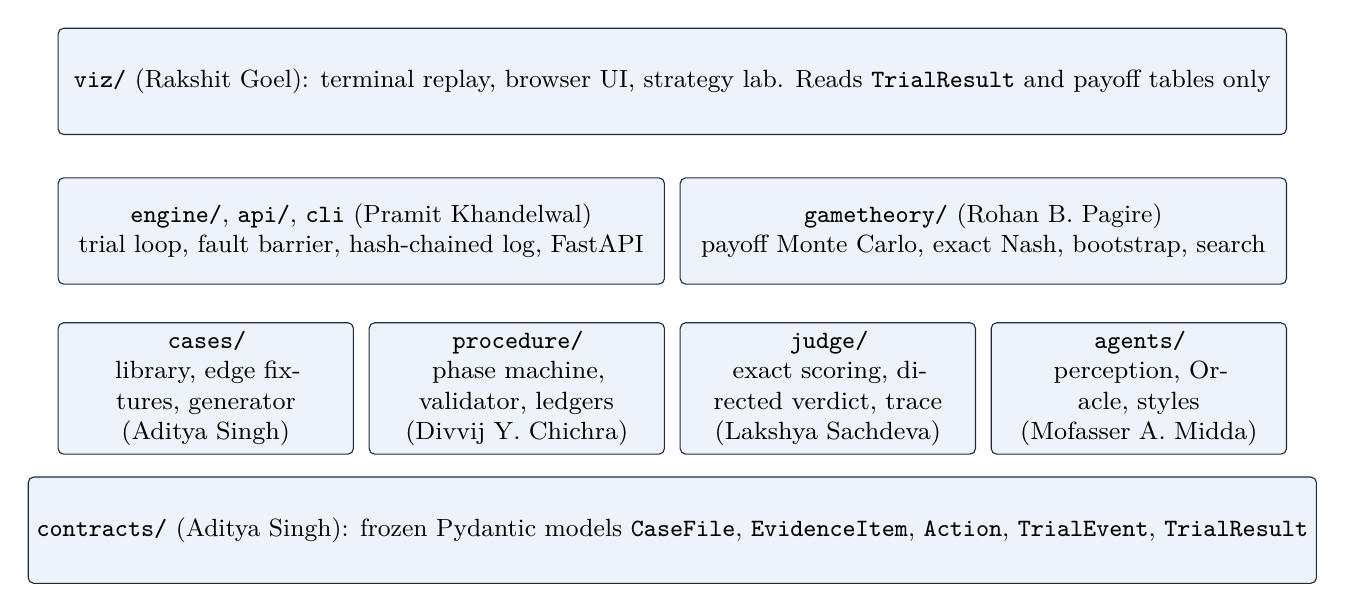
\begin{tikzpicture}[font=\small,
  box/.style={draw=navy,rounded corners=2pt,fill=accent!8,minimum height=1.35cm,align=center,inner sep=3pt},
  w1/.style={box,minimum width=15.6cm},w2/.style={box,minimum width=7.7cm},w4/.style={box,minimum width=3.75cm,text width=3.45cm}]
\node[w1] (viz) at (0,0) {\file{viz/} (Rakshit Goel): terminal replay, browser UI, strategy lab. Reads \texttt{TrialResult} and payoff tables only};
\node[w2] (eng) at (-3.95,-1.9) {\file{engine/}, \file{api/}, \file{cli} (Pramit Khandelwal)\\ trial loop, fault barrier, hash-chained log, FastAPI};
\node[w2] (gt) at (3.95,-1.9) {\file{gametheory/} (Rohan B. Pagire)\\ payoff Monte Carlo, exact Nash, bootstrap, search};
\node[w4] (cases) at (-5.925,-3.9) {\file{cases/}\\ library, edge fixtures, generator\\ (Aditya Singh)};
\node[w4] (proc) at (-1.975,-3.9) {\file{procedure/}\\ phase machine, validator, ledgers\\ (Divvij Y. Chichra)};
\node[w4] (judge) at (1.975,-3.9) {\file{judge/}\\ exact scoring, directed verdict, trace\\ (Lakshya Sachdeva)};
\node[w4] (agents) at (5.925,-3.9) {\file{agents/}\\ perception, Oracle, styles\\ (Mofasser A. Midda)};
\node[w1] (con) at (0,-5.7) {\file{contracts/} (Aditya Singh): frozen Pydantic models \texttt{CaseFile}, \texttt{EvidenceItem}, \texttt{Action}, \texttt{TrialEvent}, \texttt{TrialResult}};
\end{tikzpicture}
\caption{Package layout with the owner of each package, as assigned in the proposal. The optional \file{llm/} package (Section~\ref{sec:ai}) sits beside the core, and a test checks the core never imports it.}\label{fig:arch}
\end{figure}

\subsection{Case model and the library}
A case file holds the case type (criminal or civil), the standard of proof, the legal elements the Accuser must prove, the witnesses and the evidence items. Each item records its owner, kind (document, digital log, physical, financial record, testimony or expert), the fact it proves, its signed support $s_{ie}\in[-1,1]$ for each element (negative means it helps the Defender), the items it contradicts, its reliability, a presenting cost (1.0 for most kinds, 1.5 for testimony, 2.0 for experts) and defect flags (hearsay, unauthenticated, unlawfully obtained, undisclosed, no personal knowledge). A \emph{fact} is one distinct proposition. A validator rejects malformed or inconsistent files with the failing field named before any trial starts. The judge knows the true flags; the opposing lawyer sees a noisy signal about them (Section~\ref{sec:perception}). The library has \NCases{} cases (Section~\ref{sec:intro}); a seeded generator produces more for stress runs and for the contested-case finder.

\subsection{Trial procedure}
The trial is a finite state machine (Figure~\ref{fig:phases}). After every offered exhibit the other side gets one window: \texttt{OBJECT(ground)} or \texttt{PASS}; the judge rules and the window closes. An objection cannot itself be objected to, so objection loops cannot occur. Every phase has a turn cap, two consecutive passes count as resting, and a global event cap (400 events) forces deliberation, so every trial ends.

\begin{figure}[ht]\centering
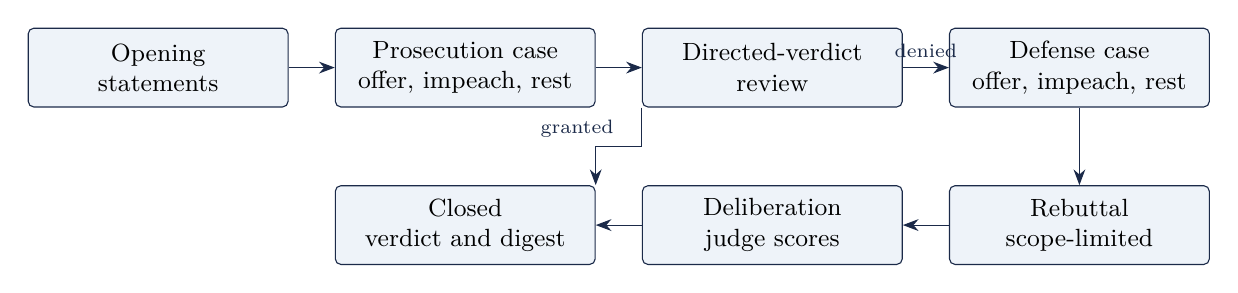
\begin{tikzpicture}[font=\small,
  st/.style={draw=navy,rounded corners=2pt,fill=accent!8,minimum height=1cm,minimum width=3.3cm,align=center,inner sep=3pt},
  ar/.style={-{Stealth[length=2mm]},navy}]
\node[st] (o) at (0,0) {Opening\\ statements};
\node[st] (p) at (3.9,0) {Prosecution case\\ offer, impeach, rest};
\node[st] (dv) at (7.8,0) {Directed-verdict\\ review};
\node[st] (d) at (11.7,0) {Defense case\\ offer, impeach, rest};
\node[st] (r) at (11.7,-2) {Rebuttal\\ scope-limited};
\node[st] (del) at (7.8,-2) {Deliberation\\ judge scores};
\node[st] (cl) at (3.9,-2) {Closed\\ verdict and digest};
\draw[ar] (o)--(p); \draw[ar] (p)--(dv); \draw[ar] (dv)--(d) node[midway,above,font=\scriptsize]{denied};
\draw[ar] (d)--(r); \draw[ar] (r)--(del); \draw[ar] (del)--(cl);
\draw[ar] (dv.south west) -- ++(0,-0.5) -| (cl.north east) node[pos=0.2,above left,font=\scriptsize]{granted};
\end{tikzpicture}
\caption{Trial phases. Rebuttal may only answer defense exhibits; it cannot add new support for an element. The Defender must move for a directed verdict, and the judge enters one on its own initiative when no admitted evidence supports an element (Section~\ref{sec:deviations}).}\label{fig:phases}
\end{figure}

Six objection grounds (hearsay, relevance, authentication, illegally obtained, late disclosure, speculation) map to named rules and are sustained only if the defect is real. A defect nobody objects to is waived, which is why objection strategy matters. An overruled objection costs the objector \(\tfrac14\) point, a procedural violation 1 point plus a fine, knowingly offering unlawful or undisclosed evidence 2 points, and three violations mean contempt. Impeaching a witness costs 1 budget unit, and, since a review finding during final preparation (E1 in \file{docs/CODE\_REVIEW.md}), it requires an exhibit that was itself offered and admitted (validator rule \texttt{V-IMPEACH-NOT-ADMITTED}).

\subsection{The deterministic judge}
The judge scores a \emph{record}: the set of admitted exhibits and the number of times each witness was impeached. It is a pure function of the record, so the same record always gives the same verdict, whatever the order of events. Arithmetic is exact (Python \texttt{Fraction}); floats appear only in display fields. The formulas below are those of \file{courtroom/judge/scoring.py}. For an admitted exhibit $i$ and legal element $e$:
\begin{align*}
S_i &= r_i\,\kappa_i, & \kappa_i &= \text{cred}_{w(i)}\cdot\tfrac12^{\,n_{w(i)}}\cdot h_{w(i)},\\
d_i &= \min\Bigl(\tfrac{9}{10},\ \sum_{j\in C(i)}\tfrac45\,\tfrac{S_j}{S_i+S_j}\Bigr), & c_{ie} &= 1 + \tfrac12\bigl(1-2^{-k_{ie}}\bigr),\\
w_{ie} &= s_{ie}\,S_i\,(1-d_i)\,c_{ie}, & L_e &= \pi + 3\sum_{i\in\text{counted}(e)} w_{ie}.
\end{align*}
Here $r_i$ is reliability, $\text{cred}_{w}$ the witness's base credibility (1 for an exhibit with no witness), $n_w$ the number of successful impeachments of the witness, $h_w=\tfrac14$ if the witness turned hostile and 1 otherwise, $C(i)$ the admitted exhibits that contradict $i$, $k_{ie}$ the number of \emph{other} facts whose admitted exhibits point the same way on $e$, and $\pi$ the prior ($-1$ criminal, $0$ civil). Only the exhibit with the largest $|w_{ie}|$ for each fact is counted, so splitting one fact into many exhibits cannot inflate the score. $L_e$ is in log-odds. The Accuser wins only if \emph{every} element clears the standard: $L_e\ge \tfrac{11}{5}$ (beyond reasonable doubt, about $0.90$), $L_e\ge\tfrac{11}{10}$ (clear and convincing, about $0.75$) or $L_e>0$ (preponderance). The test is per element, so a strong motive cannot replace proof of the act.

\emph{Why these constants.} The scale 3 means one perfect exhibit cannot convict in a criminal case ($-1+3=2<\tfrac{11}{5}$) but two independent good exhibits can. The cap $\tfrac{9}{10}$ means contradiction never erases an exhibit outright, and the corroboration bonus is capped at $50\%$. All are game parameters, moved in the sensitivity sweep.

\emph{Directed verdict.} When the prosecution rests, the Defender may move for a directed verdict; it is granted if some element is below log-odds $0$ (rule DV-1). With no admitted evidence supporting an element the judge enters it on its own initiative (DV-2). Two points differ from the proposal's text and are recorded in Section~\ref{sec:deviations}: only the strongest exhibit per fact is counted (there is no cap of four facts), and an exact tie at a non-zero bar meets it.

\subsection{Perception and the Oracle}\label{sec:perception}
A lawyer does not see an exhibit's defect flags. For each exhibit and ground it receives one binary red-flag signal with true-positive rate $a$ (the case's perception accuracy, $0.8$ by default) and false-positive rate $(1-a)/4$, and it holds the Bayesian posterior from a prior of $0.15$ that the ground applies. With $a=0.8$ a red flag raises the belief to $\tfrac{0.12}{0.1625}\approx 0.74$. Relevance is observed exactly, because the support values of an offered exhibit are public. The Oracle lets any agent query the judge's public scoring rule on a hypothetical record, which is what ``what if this were admitted'' means; it never reveals a true flag. Agents are handed a \texttt{PartyView} built by the engine; a test checks that the lookahead lawyer reads only that view and the public Oracle, and we have no equivalent source-level test for the four certified styles (a gap noted in Section~\ref{sec:discussion}).

\subsection{Agents}
A lawyer is a \texttt{StrategyProfile}: a few numbers read by one shared decision procedure, so styles differ only in risk parameters: the number of known defects it will tolerate in its own exhibit, the minimum gain that justifies spending a turn, the belief and impact above which it objects, and the share of budget held in reserve. \emph{Bold} (aggressive) offers exhibits even with up to two known defects, objects at belief $0.35$ and keeps no reserve. \emph{Careful} (conservative) offers only clean exhibits, objects only at belief $0.70$ and impact $0.25$, and keeps $25\%$ in reserve. \emph{Smart} (adaptive) picks the move of highest expected utility under its beliefs and learns the opponent's objection rate with a Beta posterior. \emph{Wild} (reckless) plays random legal moves and sometimes breaks a rule; the proposal's Mixed$(p)$ remains in the code but is not in the four-by-four game (Section~\ref{sec:deviations}). A \emph{Chaos} agent, used only in robustness tests, plays illegal actions at random. A \emph{lookahead} lawyer (depth-limited alpha-beta) and an optional language-model lawyer exist as labelled exhibitions and are never in a certified table.

\subsection{The game layer and the analyses}\label{sec:analyses}
Each analysis below is computed from the stored results, uses the same engine and judge as the demo, and states what it assumes.
\begin{description}
\item[Payoff Monte Carlo.] Every pair of the four styles is played on the same seeds (common random numbers) to estimate a $4\times4$ bimatrix of mean utilities, with standard errors.
\item[Exact Nash solver.] Pure equilibria by scanning, mixed ones by support enumeration over \texttt{Fraction}s, iterated elimination of dominated strategies, and an independent verifier that no side gains by deviating. A case is labelled \emph{pure}, \emph{mixed} or \emph{dominance-solvable}.
\item[Bootstrap stability.] The seed set is resampled with replacement and the game re-solved; the stability of a label is the share of resamples that give the same label.
\item[Sensitivity.] The rulebook's constants (costs, sanctions, the scale $3$, the prior defect rate and the standards of proof) are moved by $\pm25\%$ and the library is re-solved. The ``almost certain'' bar is also set between $80\%$ and $95\%$.
\item[Does strategy matter?] For each case every pairing of Bold, Careful and Smart is played over several seeds; the \emph{pairing spread} is the best Accuser win rate minus the worst, and the \emph{seed coin-flip} is the average of $2\min(p,1-p)$. The words ``decided by the evidence'' or ``by the lawyers'' only label these two numbers.
\item[Best-response search (double oracle).] Starting from the four styles on each side, up to four rounds: solve the game; for each side search the five profile parameters (a seeded random search, then local refinement) for the profile earning most against the other side's equilibrium mix on training seeds; re-test it on held-out seeds with a paired comparison; keep it only above two standard errors; solve again. Each kept profile is confirmed on a third seed set. No language model is involved.
\item[Classic-game classifier.] A two-by-two corner of a payoff table is named (prisoner's dilemma, stag hunt, battle of the sexes, chicken, matching pennies) by the \emph{order} of its payoffs, treating differences under two standard errors as ties. It reads pairs of styles only.
\item[Pareto efficiency and security values.] Exact Pareto and maximin computations (vertex enumeration in rationals); the minimax theorem is checked on the win-probability game, which is constant-sum.
\item[Minimax and alpha-beta.] The trial as a tree, with plain minimax, alpha-beta and alpha-beta with move ordering, on the engine's own rules. This is an \emph{open-file relaxation}: both sides see every exhibit and flaw (no perception noise), and the payoff is made zero-sum (Accuser utility minus Defender utility). It is not the game the certified analysis solves.
\item[Contested-case finder and tipping point.] The finder scores generated cases with the does-strategy-matter measure and solves the most contested; the tipping point is the smallest change to one exhibit's reliability or one witness's credibility that flips a verdict, found by re-scoring the record with the judge itself.
\end{description}

\subsection{Engine, API, demo and reproducibility}\label{sec:repro}
The engine runs a trial, catches agent faults, and keeps a hash-chained event log; each trial ends in a digest, and \texttt{python -m courtroom verify} runs a case twice and compares digests and the chain. The FastAPI server exposes trials, games, the analyses and case validation; heavy endpoints are bounded. The web demo is plain JavaScript. The hosted copy is static: it plays the \ReplayTotal{} recorded trials in a bundle and shows the stored analysis, and says so; only the local server computes fresh trials. Every spoken line is pre-recorded with a fixed voice per character, so the voice does not depend on the device. \file{PROVENANCE.md} gives one command per claim, and a test regenerates the documents and fails if one is stale.

\section{Results and evaluation}\label{sec:results}
All numbers in this section are generated from \file{results/}, from the evaluation measurements in \file{report/generated/eval\_plan.json} (\file{scripts/eval\_plan.py}) or from git, by \file{report/build\_report.py}. No case, parameter or seed was changed after seeing a result.

\subsection{The proposal's evaluation plan, row by row}
Table~\ref{tab:evalplan} takes each row of the proposal's evaluation plan (proposal Section~8) and says whether its ``done when'' criterion was met, with the evidence.

\begin{table}[ht]\centering\footnotesize
\caption{The proposal's evaluation plan against what was measured.}\label{tab:evalplan}
\begin{tabularx}{\textwidth}{@{}p{1.9cm}p{3.6cm}p{1.3cm}X@{}}
\toprule
\textbf{Check} & \textbf{Done when (proposal)} & \textbf{Met?} & \textbf{Evidence}\\
\midrule
Correctness & All fixtures match and every known equilibrium is found exactly. & Yes & \TestsCorrectness{} tests pass (\TestsFailedCorrectness{} fail): hand-computed judge fixtures, including a record that lands exactly on the clear-and-convincing bar; property tests (determinism, order independence, monotonicity, no single-item conviction); the solver on the prisoner's dilemma, battle of the sexes, matching pennies and rock-paper-scissors; a verifier that rejects non-equilibria.\\
Robustness & Every fixture gives its expected outcome; no crash or broken invariant; all replay hashes identical. & Yes, with one expectation not met as written & Four edge fixtures are library cases (Table~\ref{tab:edge}); every verdict is as expected, but in the defense-only fixture the Defender spent \DefenseOnlySpent{} budget units where the proposal expected none (the cost of the directed-verdict motion the Defender must now make, D5); the malformed case file and the illegal or out-of-turn action are tested as rejections (contract tests, the validator rule table, contempt after three violations). Fuzz: 100 generated cases $\times$ 25 pairings (Chaos and Mixed included) $=$ \StressTrials{} trials, \StressCrashes{} crashes, \StressInvariant{} broken invariants, and \StressReplays{} of \StressTrials{} replays identical. All \ReplaySame{} of \ReplayTotal{} recorded trials reproduce their pinned digest and \ReplayChain{} hash chains verify. \TestsRobustness{} tests in the robustness group pass.\\
Analysis & $4\times4$ payoff matrices over 200 common seeds per cell, with standard errors and 200 bootstrap resamples; each case labelled pure, mixed or dominance-solvable with the label's stability. & Yes, after a re-run & The first certified runs used \BootOldSeeds{} seeds per cell. We re-ran the payoff tables, the bootstrap and the classic-game labels at \BootSeeds{} seeds and \BootResamples{} resamples with the documented scripts (Table~\ref{tab:seeds}); Table~\ref{tab:bootstrap} gives each case's label and stability, and the stored payoff intervals bound each cell.\\
Sensitivity & Sanctions, costs, the scale 3 and each standard varied by $\pm25\%$; report which conclusions survive. & Yes, with fewer seeds & \SensVariations{} settings re-solved on \SensSeeds{} seeds per cell (fewer than the other analyses, to keep the run to minutes); \SensRobust{} cases never changed label, \SensFragile{} changed under at least one setting (Table~\ref{tab:sens}).\\
Live demo & Any case, pairing and seed stepped and replayed with the judge trace; a trial runs in under 1\,s, all six edge fixtures run cleanly live, and an examiner-made case never crashes the demo; works offline from a bundle. & Yes & Slowest of \TimedTrials{} timed pairings: \TrialMaxMs{}\,ms (median \TrialMedianMs{}\,ms). The four edge cases play live; the other two fixtures are input rejections. \TestsLiveDemo{} tests of the API, the CLI, the editor and the recorded bundle pass, including absurd editor input (empty, huge, negative, non-numeric and script-tag values) typed into a real browser. The bundle makes the demo run offline.\\
\bottomrule
\end{tabularx}
\end{table}

\begin{table}[ht]\centering
\caption{The four edge fixtures that are library cases, as measured (Bold against Careful, seed 0). The proposal fixed the expected outcome before any code: the empty docket and the defense-only case end at the directed-verdict review (DV-2) with the Defender winning, (the proposal also expected the Defender to spend nothing in the defense-only case; it spent the cost of the motion, see Table~\ref{tab:evalplan}); two equally credible, mutually exclusive witnesses cancel and the burden of proof decides for the Defender; and when every exhibit is defective, each objected exhibit is excluded and its presenter sanctioned, and the verdict equals the verdict on the admitted record.}\label{tab:edge}
% generated by report/build_report.py: do not edit
{\footnotesize
\begin{tabularx}{\textwidth}{@{}>{\raggedright\arraybackslash}p{3.7cm}>{\raggedright\arraybackslash}p{3cm}>{\raggedright\arraybackslash}p{4.6cm}>{\raggedright\arraybackslash}p{2.6cm}@{}}
\toprule
\textbf{Edge fixture} & \textbf{Verdict (Bold vs Careful, seed 0)} & \textbf{Rules fired} & \textbf{Budget spent (Accuser / Defender)} \\
\midrule
edge-defense-only & directed acquittal & DV-2, ELEM-1, STD-1, VER-DV & 0 / 0.5 \\
edge-empty-docket & directed acquittal & DV-2, ELEM-1, STD-1, VER-DV & 0 / 0.5 \\
edge-mutual-exclusion & not liable & ADM-WAIVER, DV-2, ELEM-1, OBJ-HEARSAY, SANCTION-OVR, STD-1 & 2 / 1.5 \\
edge-poisoned-tree & not guilty & ADM-WAIVER, DV-2, ELEM-1, OBJ-AUTH, OBJ-DISCLOSURE, OBJ-EXCLUSIONARY & 5.5 / 2 \\
\bottomrule
\end{tabularx}}

\end{table}

Two proposal items were stretch goals: replicator dynamics (implemented in \file{gametheory/dynamics.py}) and an expectimax agent (replaced by a depth-limited alpha-beta \emph{lookahead} lawyer that weighs an opponent's objection by its own belief; an exhibition, not certified). The hash-chained log and the terminal replay (\texttt{python -m courtroom run}) were kept.

\subsection{Does strategy matter here?}
Table~\ref{tab:matters} and Figure~\ref{fig:matters} measure, for each case, how far the lawyers' styles and the seed move the Accuser's win rate (\MSeeds{} seeds, all nine pairings of Bold, Careful and Smart). The lawyers move the verdict in \NMove{} of \NCases{} cases (\NLawyers{} decided by the lawyers and \NPartly{} partly); the other \NEvidence{} are decided by the evidence alone, so in those no style and no seed changes the verdict and a strategy comparison has nothing to find. This was the first thing we measured and it was uncomfortable: it is why the demo script names which cases to use to show strategy mattering and which to present as plain trials.

\begin{table}[ht]\centering\caption{Does strategy matter? (Generated from \file{results/matters.json} and \file{matters\_surprises.json}.)}\label{tab:matters}
% generated by report/build_report.py: do not edit
{\small
\begin{tabularx}{\textwidth}{@{}>{\raggedright\arraybackslash}p{4cm}>{\raggedright\arraybackslash}p{2.9cm}rr>{\raggedright\arraybackslash}p{2.9cm}@{}}
\toprule
\textbf{Case} & \textbf{Verdict (plain rules)} & \textbf{Lawyers move it by} & \textbf{Seed coin-flip} & \textbf{Verdict (surprises on)} \\
\midrule
Aurora Protocol Flash-Loan Exploit & Decided by the evidence & 0\% & 0\% & Decided by the evidence \\
The Broken Bike & Decided by the lawyers & 50\% & 22\% & Partly the lawyers \\
The Missing Cookies & Decided by the evidence & 0\% & 0\% & Decided by the evidence \\
Prosecution Brings Only Exculpatory Material & Decided by the evidence & 0\% & 0\% & Decided by the evidence \\
The Empty Docket & Decided by the evidence & 0\% & 0\% & Decided by the evidence \\
Mutually Exclusive Testimony & Decided by the evidence & 0\% & 0\% & Decided by the evidence \\
Fruit of the Poisonous Tree & Partly the lawyers & 25\% & 17\% & Partly the lawyers \\
The Dug-Up Garden & Decided by the evidence & 0\% & 0\% & Decided by the evidence \\
Helix Dynamics Trade-Secret Exfiltration & Decided by the lawyers & 100\% & 17\% & Decided by the lawyers \\
AV-7 Crosswalk Collision & Decided by the lawyers & 100\% & 8\% & Decided by the lawyers \\
\bottomrule
\end{tabularx}}

\end{table}
\begin{figure}[ht]\centering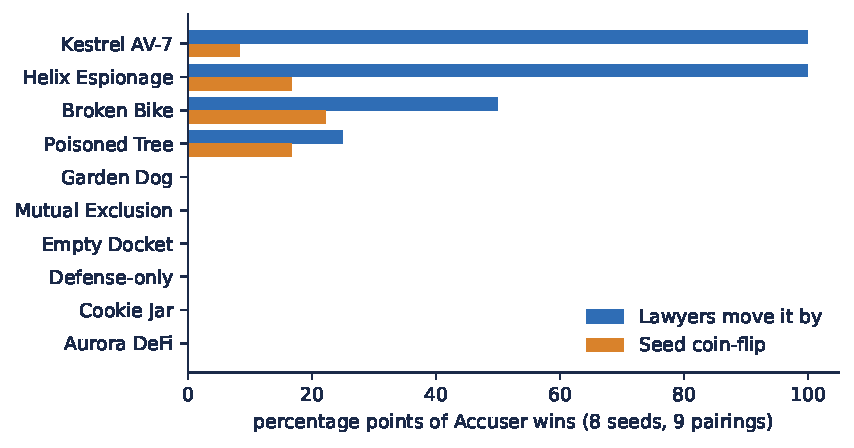
\includegraphics[width=0.78\textwidth]{figures/fig_matters.pdf}\caption{How far the lawyers and the seed move the Accuser's win rate in each case (plain rules).}\label{fig:matters}\end{figure}

\subsection{How stable are the equilibrium labels?}
Each game was re-solved on \BootResamples{} resamples of \BootSeeds{} seeds (Table~\ref{tab:bootstrap}, Figure~\ref{fig:bootstrap}). With plain rules, \BootBelowPlain{} cases came back less than $80\%$ of the time; the lowest is \BootWorstPlainCase{} at \BootWorstPlain{}. With courtroom surprises on, \BootBelowSurprises{} case falls below $80\%$: \BootWorstSurprisesCase{} at \BootWorstSurprises{}.

The earlier run at \BootOldSeeds{} seeds looked weaker: \BootOldBelow{} cases were below $80\%$ under plain rules (\BootOldWorstCase{}, \BootOldWorst{}; \BootOldSecondCase{}, \BootOldSecond{}). Doubling the seeds raised those, which suggests the weak stability at \BootOldSeeds{} seeds was partly sampling noise. We report both runs because the earlier one is in the git history (Section~\ref{sec:discussion}).

\begin{table}[ht]\centering\caption{Equilibrium label and its bootstrap stability.}\label{tab:bootstrap}
% generated by report/build_report.py: do not edit
{\small
\begin{tabularx}{\textwidth}{@{}>{\raggedright\arraybackslash}p{5cm}lrlr@{}}
\toprule
\textbf{Case} & \textbf{Label (plain)} & \textbf{Stability} & \textbf{Label (surprises on)} & \textbf{Stability} \\
\midrule
Aurora Protocol Flash-Loan Exploit & pure & 100.0\% & pure & 100.0\% \\
The Broken Bike & mixed & 87.0\% & pure & 83.0\% \\
The Missing Cookies & pure & 100.0\% & dominance-solvable & 100.0\% \\
Prosecution Brings Only Exculpatory Material & pure & 100.0\% & pure & 100.0\% \\
The Empty Docket & pure & 100.0\% & pure & 100.0\% \\
Mutually Exclusive Testimony & pure & 100.0\% & pure & 100.0\% \\
Fruit of the Poisonous Tree & mixed & 100.0\% & mixed & 100.0\% \\
The Dug-Up Garden & pure & 100.0\% & pure & 60.5\% \\
Helix Dynamics Trade-Secret Exfiltration & mixed & 99.5\% & mixed & 100.0\% \\
AV-7 Crosswalk Collision & mixed & 97.5\% & dominance-solvable & 88.5\% \\
\bottomrule
\end{tabularx}}

\end{table}
\begin{figure}[ht]\centering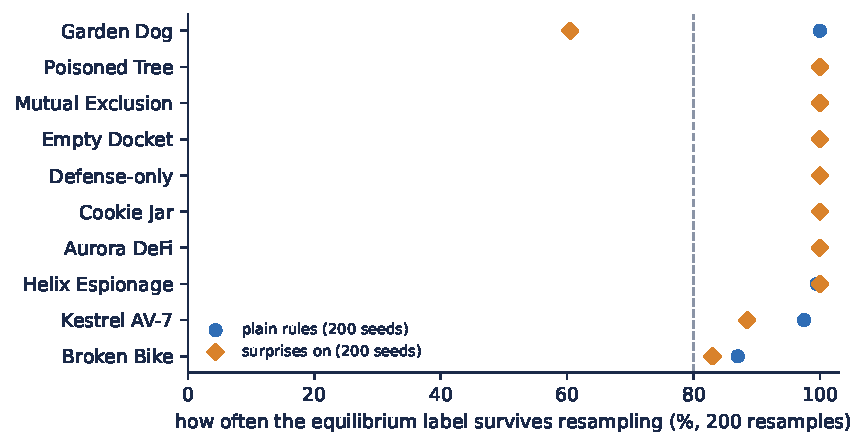
\includegraphics[width=0.78\textwidth]{figures/fig_bootstrap.pdf}\caption{Bootstrap stability of each case's equilibrium label; the dashed line is $80\%$.}\label{fig:bootstrap}\end{figure}

\subsection{Does the rulebook's choice of constants decide the conclusions?}
Table~\ref{tab:sens} counts how many cases changed label when each constant was moved. The constant that changes most labels is the prior defect rate (\SensPriorChanges{} label changes), the lawyers' prior that any ground applies to an exhibit; this is a belief inside the agents, not a rulebook constant, and it is a modelling choice we did not measure.

\begin{table}[ht]\centering\caption{Label changes under the sensitivity sweep.}\label{tab:sens}
% generated by report/build_report.py: do not edit
{\small
\begin{tabularx}{\textwidth}{@{}lrr@{}}
\toprule
\textbf{Constant moved} & \textbf{Label changes (plain)} & \textbf{Label changes (surprises on)} \\
\midrule
LLR SCALE & 1 & 2 \\
PRIOR DEFECT RATE & 6 & 6 \\
beyond reasonable doubt & 1 & 2 \\
costs & 1 & 2 \\
sanctions & 1 & 3 \\
standards of proof & 0 & 0 \\
\bottomrule
\end{tabularx}}

\end{table}

\subsection{Can a better lawyer be found?}
The best-response search found a lawyer that beats the four hand-written styles in \NBeaten{} of \NSearches{} searches (each searched case is run with surprises off and on); the largest gain is \BestGain{} utility per trial for the Defender in \BestCase{} with plain rules. Every kept profile was confirmed on seeds that played no part in finding or accepting it (Table~\ref{tab:oracle}, Figure~\ref{fig:oracle}). ``No better lawyer found'' means none was found in a five-parameter family within a budget of \OracleBudget{} profiles per side per round; it is evidence, not proof.

\begin{table}[ht]\centering\caption{Best-response search results.}\label{tab:oracle}
% generated by report/build_report.py: do not edit
{\small
\begin{tabularx}{\textwidth}{@{}>{\raggedright\arraybackslash}p{4.9cm}lrr>{\raggedright\arraybackslash}p{3.5cm}@{}}
\toprule
\textbf{Case} & \textbf{Surprises} & \textbf{Kept} & \textbf{Confirmed on fresh seeds} & \textbf{Gain per trial vs the old equilibrium} \\
\midrule
The Broken Bike & off & 1 & 1 of 1 & defense: +0.88 \\
The Broken Bike & on & 0 & 0 of 0 & none \\
Helix Dynamics Trade-Secret Exfiltration & off & 2 & 2 of 2 & defense: +1.59 \\
Helix Dynamics Trade-Secret Exfiltration & on & 2 & 2 of 2 & defense: +0.91 \\
AV-7 Crosswalk Collision & off & 0 & 0 of 0 & none \\
AV-7 Crosswalk Collision & on & 1 & 1 of 1 & prosecution: +1.22 \\
\bottomrule
\end{tabularx}}

\end{table}
\begin{figure}[ht]\centering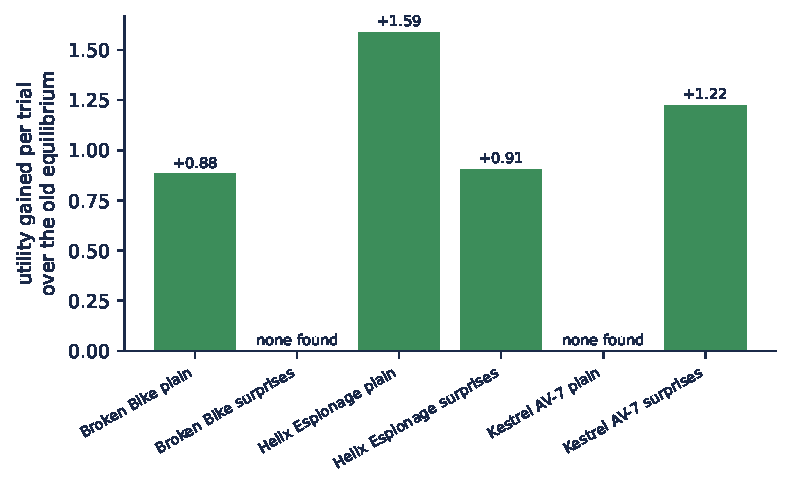
\includegraphics[width=0.78\textwidth]{figures/fig_oracle.pdf}\caption{Utility gained per trial by the best discovered lawyer over the old equilibrium.}\label{fig:oracle}\end{figure}

\subsection{The lecture concepts, computed on our own games}
Table~\ref{tab:lectures} lists each lecture concept, what our data says and the relaxation or limit it carries. Of the games the brief named, none of the prisoner's dilemma, stag hunt, battle of the sexes or chicken was found among the \ClassicCorners{} two-by-two corners of the library (\ClassicFoundTotal{} found), and \SearchKept{} survived the search over \SearchTried{} generated cases: \SearchLookedDilemma{} corners looked like a prisoner's dilemma and \SearchLookedStag{} like a stag hunt when read as exact numbers, but none kept its name under the full tolerance on fresh seeds. Matching pennies appears in \MatchingPennies{} corners. The minimax theorem held in \TheoremHolds{} of \TheoremTotal{} win-probability games. The trial tree was solved exactly in \TreeSolved{} of \TreeTotal{} cases and plain minimax, alpha-beta and alpha-beta with move ordering agreed in every one (Figure~\ref{fig:tree}). The lookahead lawyer beat the four-style equilibrium in \LookBeats{} of \NCases{} cases (\LookBeatsCase{}). ``Not found'' is a statement about the library and the cases tried, not a proof that no such case exists; no case was retuned to make a classic game appear.

\begin{table}[ht]\centering\caption{Lecture concepts: where each is computed and what our data says (generated).}\label{tab:lectures}
% generated by report/build_report.py: do not edit
{\footnotesize
\begin{tabularx}{\textwidth}{@{}>{\raggedright\arraybackslash}p{2.8cm}>{\raggedright\arraybackslash}p{5.2cm}>{\raggedright\arraybackslash}p{6cm}@{}}
\toprule
\textbf{Lecture concept} & \textbf{What our data says} & \textbf{Relaxation or limit} \\
\midrule
Prisoner's dilemma & \textbf{Not found.} 0 of 360 corners in the library, and 0 kept after searching 395 generated cases. & Only pairs of styles (2×2 corners of the 4×4 table). A gap under two standard errors is a tie, and a game needing a strict order where there is a tie is called none of the classic games. \\
Stag hunt & \textbf{Not found.} 0 of 360 corners in the library, and 0 kept after searching 395 generated cases. & Risk is read from each play's worst case (a security-level notion), not from risk dominance. \\
Battle of the sexes (Bach or Stravinsky) & \textbf{Not found.} 0 of 360 corners in the library, and 0 kept after searching 395 generated cases. & Needs two pure equilibria that the sides rank differently. \\
Chicken & \textbf{Not found.} 0 of 360 corners in the library, and 0 kept after searching 395 generated cases. & The same two-equilibria shape with a full strict order of four outcomes. \\
Matching pennies & 16 corners (plain), 14 (surprises on) & Named when no pure equilibrium survives the tolerance; the sides need not be zero-sum. \\
Pareto optimality & Some equilibrium dominated for both sides in 1 of 10 cases (plain), 1 (surprises on). & Compared on mean payoffs over pure pairs of styles; a mixed equilibrium is compared by its expected payoffs, and mixing across cells together is not considered. \\
Minimax and the minimax theorem & Maximin = minimax = Nash value in 20 of 20 win-probability games. & Holds only for the constant-sum win-probability game. The real game is general-sum, so there the security value is only a floor. \\
Minimax on the trial tree & 17 of 18 cases solved exactly. & An open-file relaxation: both sides see all exhibits and flaws, no perception noise, and a zero-sum payoff (Accuser utility minus Defender utility). The real game has hidden information and is not zero-sum. \\
Alpha-beta pruning & Same value as plain minimax in all 15 cases where both finished, with move ordering cutting the nodes visited as shown in the table. & Pruning is exact; the saving depends on the case and on the ordering heuristic. \\
Thinking ahead (depth-limited alpha-beta) & Beat the four-style equilibrium in 1 of 10 cases (plain) and 1 (surprises on). & Exhibition, not certified. It uses only its own view and the public oracle, assumes the worst reply, and scores positions with a heuristic. \\
\bottomrule
\end{tabularx}}

\end{table}
\begin{figure}[ht]\centering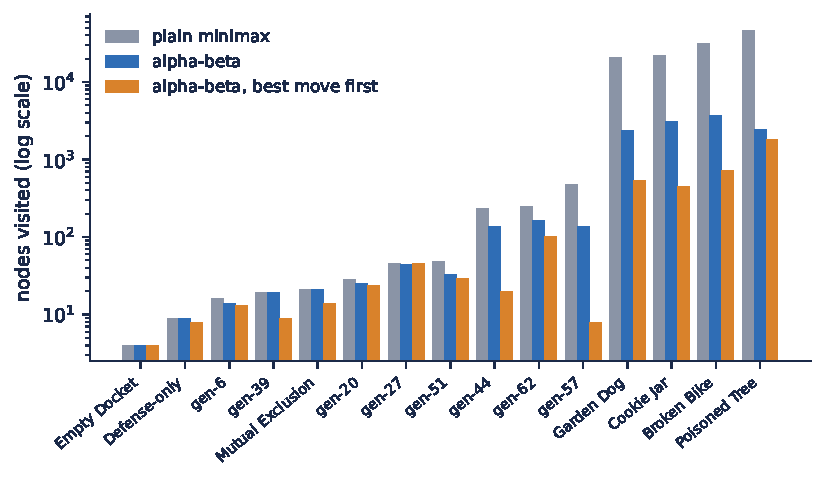
\includegraphics[width=0.85\textwidth]{figures/fig_tree.pdf}\caption{Nodes visited by plain minimax, alpha-beta and alpha-beta with move ordering on the cases where all three finished (log scale).}\label{fig:tree}\end{figure}

\subsection{An example payoff table}
Figure~\ref{fig:payoff} shows the Accuser's win rate for each pair of styles in one case where the lawyers matter. The equilibrium of such a table is what the analyses above label.

\begin{figure}[ht]\centering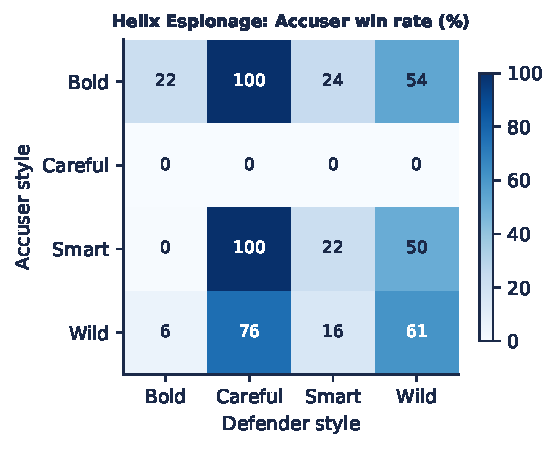
\includegraphics[width=0.5\textwidth]{figures/fig_payoff.pdf}\caption{The Accuser's win rate (\%) for every pair of the four styles in a case the lawyers decide (\BootSeeds{} seeds per cell).}\label{fig:payoff}\end{figure}

\subsection{Seeds per cell actually used}
\begin{table}[ht]\centering\caption{Seeds per cell, read from the result files.}\label{tab:seeds}
% generated by report/build_report.py: do not edit
{\small
\begin{tabularx}{\textwidth}{@{}>{\raggedright\arraybackslash}p{6cm}>{\raggedright\arraybackslash}p{5cm}r@{}}
\toprule
\textbf{Analysis} & \textbf{File} & \textbf{Seeds per cell} \\
\midrule
Bootstrap of the equilibrium label & \texttt{results/bootstrap.json} & 200 \\
Classic-game labels & \texttt{results/classic.json} & 200 \\
Pareto and security & \texttt{results/efficiency.json} & 200 \\
Rulebook sensitivity & \texttt{results/sensitivity.json} & 16 \\
Does strategy matter & \texttt{results/matters.json} & 8 \\
Lookahead comparison & \texttt{results/lookahead.json} & 40 \\
\bottomrule
\end{tabularx}}

\end{table}

\section{Discussion and limitations}\label{sec:discussion}

\subsection{What the results say}
\emph{Most cases are decided by the evidence.} In \NEvidence{} of \NCases{} cases the verdict does not move with the lawyers' styles or the seed. We did not expect this and it limits the strategic story: a game-theoretic comparison of styles only has something to find in the \NMove{} cases the lawyers move. Among the three flagship cases written to showcase strategy, the one decided by the evidence is: \FlagshipEvidence{}; we report that as it is.

\emph{Conclusions depend on the seed count and on one belief.} At \BootOldSeeds{} seeds two cases looked unstable; at \BootSeeds{} they do not, so a comparison with few seeds can mislead, and the proposal's 200 seeds were justified. The label changes most under the lawyers' prior defect rate (\SensPriorChanges{} changes, Table~\ref{tab:sens}), a belief inside the agents that we chose and did not measure. Sensitivity itself was run on only \SensSeeds{} seeds per cell.

\emph{The four styles can be beaten, in some cases.} The search found better lawyers in \NBeaten{} of \NSearches{} runs, so ``Bold, Careful, Smart and Wild'' is a hand-picked menu, not the space of strategies; the finding that the equilibrium of the four-style game is not an equilibrium of the larger game matters for how it is read.

\emph{Not found.} No prisoner's dilemma, stag hunt, battle of the sexes or chicken appears in the library or among the generated cases searched. The classifier looks at pairs of styles, so a game that needs a third style or a mixed strategy is invisible to it.

\subsection{Limitations}
\begin{itemize}
\item \textbf{A stylised legal model.} The thresholds, constants and costs are game parameters, not legal probabilities. The system is a teaching demo, not a model of real court procedure and not a guilt predictor.
\item \textbf{Synthetic cases written by us.} Their evidence values are modelling choices. The library was not tuned to produce any reported result, but it was written before the measurements by people who knew what they wanted to show.
\item \textbf{Surprise chances are chosen, not observed.} Results with courtroom surprises on read as ``if this kind of luck exists''.
\item \textbf{Relaxations.} The tree search assumes both sides see everything and the payoff is zero-sum, and covers only the cases small enough to finish; the minimax theorem holds only for the constant-sum win-probability game, not for the real general-sum game; the classifier reads pairs of styles at a tolerance of two standard errors.
\item \textbf{Extras, labelled.} The lookahead lawyer and the optional language-model layer are exhibitions outside every certified result. The language-model layer contradicts the proposal's ``no language model'' positioning if read as part of the core, so it is optional, off by default, never imported by the core (a test checks), and never in a certified table.
\item \textbf{Several comparisons are made.} The search tries candidates over rounds, so a lone result just above two standard errors is weak evidence; every kept profile is confirmed on fresh seeds for that reason.
\item \textbf{Where the proposal and the code differ} is in Section~\ref{sec:deviations}, including two differences in the judge's formula that we found while writing this report (D7, D8) and did not change, because every certified result depends on the judge.
\item \textbf{Test gap.} Only the lookahead lawyer has a source-level test that it reads nothing but its own view and the public Oracle; the four certified styles do not.
\item \textbf{The hosted site replays.} The static copy plays recorded trials and the stored analysis; only the local server computes fresh trials.
\end{itemize}

\subsection{A code review before the demo}
Before the demo we ran a structured code review of the whole project: \ReviewTotal{} findings in total, of which \ReviewFixed{} were fixed, \ReviewDeferred{} deferred with a reason and \ReviewRejected{} rejected. The most serious was a demo script that pointed the presenter to a docket group that did not exist; the most consequential for results was that the engine let a lawyer impeach a witness with an exhibit that had never been admitted (E1). Fixing E1 changed \EOneDigests{} of the \EOneTrials{} recorded trials and \EOneFlipped{} recorded verdicts, and required re-running the certified analyses; it is recorded as deviation D6 and the pinned digests were re-pinned deliberately.

\subsection{Honest reflection on the process}
We state these facts about how the work was done, because the course asks for an honest account.
\begin{itemize}
\item \textbf{Two histories describe the same code, and they disagree about when it was written.} The \emph{official course repository} (\file{course/main}, Table~\ref{tab:course}) has \CourseCommits{} non-merge commits by \CourseAuthors{} author names between \CourseFirst{} and \CourseLast{}, with between \CourseMinPerDay{} and \CourseMaxPerDay{} commits on each of \CourseDays{} days, and it shows each package being added in turn: contracts and cases on \CourseFirstContracts{}, procedure on \CourseFirstProcedure{}, the judge on \CourseFirstJudge{}, agents on \CourseFirstAgents{}, the engine on \CourseFirstEngine{} and the game theory on \CourseFirstGametheory{}. The lineage this report was written from (\file{final-integration}) starts with one commit on \LumpDate{} that already contains the whole core, and \CourseSame{} of the \CourseCore{} core source files in that commit are byte-identical to the official repository's final versions. Git alone cannot say which timeline is the working history. \todo{TEAM TO EXPLAIN how the official history was produced, for example whether the commits were re-created from earlier local work, because the rubric's commit-history criterion and the viva both depend on it}
\item \textbf{This branch's lineage is uneven.} It has \NCommits{} non-merge commits by \NAuthors{} git author names over \NCommitDays{} days between \FirstCommit{} and \LastCommit{} (Table~\ref{tab:git}); most later work was done by one author, with AI assistance (Section~\ref{sec:ai}), and much of it in the last weeks before the deadline.
\item \textbf{The planned weekly gates were not tracked in git.} Table~\ref{tab:milestones} lists when each milestone first appears in git; it does not show weekly commits or cross-reviews by every member.
\item \textbf{What would have helped:} each member committing their own package in their own name through the semester, with a visible review of a teammate's package. The remedy now is real work in each member's name (their contribution paragraph, their viva notes, tests of their package), not rewriting history or authorship.
\end{itemize}

\begin{table}[ht]\centering\caption{The official course repository (\file{course/main}): commits by author name and the areas touched. Author names are as recorded; mapping a name to a team member is for the team to confirm.}\label{tab:course}
% generated by report/build_report.py: do not edit
{\footnotesize
\begin{tabularx}{\textwidth}{@{}>{\raggedright\arraybackslash}p{5cm}r>{\raggedright\arraybackslash}p{8cm}@{}}
\toprule
\textbf{Author name in the official repository} & \textbf{Commits} & \textbf{Files touched by area (count)} \\
\midrule
binarycoder3012 & 19 & viz 146, judge 5, README.md 3, docs 1 \\
RakshitGoel007 & 16 & viz 24 \\
PramitKH26 & 14 & api 4, engine 4, courtroom 3, tests 3 \\
Divvij0202 & 10 & viz 142, procedure 3, tests 1 \\
Aditya & 8 & viz 135, cases 4, tests 3, contracts 2 \\
Mofasser Arafat & 8 & viz 135, agents 7, tests 2 \\
rohanp-965 & 6 & gametheory 4, scripts 1, tests 1, viz 1 \\
Lakshya Sachdeva & 1 & README.md 1 \\
\bottomrule
\end{tabularx}}

\end{table}
\begin{table}[ht]\centering\caption{Commits by git author name over all local branches (no merges), and the areas of the repository each touched. Names are the git author names as recorded; mapping a name to a team member is for the team to confirm.}\label{tab:git}
% generated by report/build_report.py: do not edit
{\footnotesize
\begin{tabularx}{\textwidth}{@{}>{\raggedright\arraybackslash}p{3.2cm}r>{\raggedright\arraybackslash}p{3.6cm}>{\raggedright\arraybackslash}p{6cm}@{}}
\toprule
\textbf{Git author name} & \textbf{Commits} & \textbf{First to last} & \textbf{Files touched by area (count)} \\
\midrule
Pramit Khandelwal & 72 & 2026-10-17 to 2026-11-17 & viz 119, tests 95, results 56, llm 35, scripts 29, docs 27 \\
binarycoder3012 & 31 & 2026-10-02 to 2026-11-17 & viz 720, README.md 6, judge 5, scripts 4, docs 3, tests 3 \\
RakshitGoel007 & 16 & 2026-10-22 to 2026-11-10 & viz 24 \\
PramitKH26 & 14 & 2026-10-11 to 2026-11-08 & api 4, engine 4, tests 3, cli 2, viz 2, courtroom (top level) 1 \\
Divvij0202 & 11 & 2026-09-30 to 2026-11-11 & viz 147, procedure 3, tests 1 \\
Mofasser Arafat & 8 & 2026-10-17 to 2026-11-06 & viz 135, agents 7, tests 2 \\
Aditya & 8 & 2026-10-11 to 2026-11-05 & viz 135, cases 4, tests 3, contracts 2, .gitignore 1, README.md 1 \\
rohanp-965 & 6 & 2026-10-19 to 2026-11-09 & gametheory 4, scripts 1, tests 1, viz 1 \\
Lakshya Sachdeva & 1 & 2026-10-02 to 2026-10-02 & README.md 1 \\
savage2006 & 1 & 2026-09-27 to 2026-09-27 & tests 9, viz 6, agents 5, judge 5, engine 4, gametheory 4 \\
\bottomrule
\end{tabularx}}

\end{table}
\begin{table}[ht]\centering\caption{When key artefacts first appear in git, against the proposal's gates (G1 16 Oct, G2 23 Oct, G3 6 Nov).}\label{tab:milestones}
% generated by report/build_report.py: do not edit
{\small
\begin{tabularx}{\textwidth}{@{}>{\raggedright\arraybackslash}p{2.4cm}X@{}}
\toprule
\textbf{Date} & \textbf{What (first appearance in git, or a planned gate)} \\
\midrule
2026-09-27 & Core engine in one commit: contracts, cases, procedure, judge, agents, Nash solver, engine, API, CLI, web UI \\
2026-10-16 & Gate G1 planned (one case runs end to end); first evidence in git 2026-09-27 (courtroom/engine/trial.py): before the gate \\
2026-10-23 & Gate G2 planned (integrated demo on all three cases); first evidence in git 2026-09-27 (courtroom/viz/web/data/bundle.js): before the gate \\
2026-11-06 & Gate G3 planned (parameters frozen, results reproduced); first evidence in git 2026-11-12 (results/bootstrap.json): 6 days after the gate \\
2026-11-11 & Strategy lab page \\
2026-11-12 & Bootstrap stability of the equilibrium label \\
2026-11-12 & Does-strategy-matter measurement \\
2026-11-12 & First certified result file \\
2026-11-12 & Pinned digests of the recorded trials \\
\bottomrule
\end{tabularx}}

\end{table}

\section{Individual contributions}\label{sec:contrib}
The source of truth for \emph{who was responsible for what} is the proposal's ownership table (Section~11 of the proposal). The source for \emph{what the repository shows} is git (Table~\ref{tab:git}). Where git does not show a member's work we say so and leave a marked placeholder for that member to write in their own words. Placeholders are in \todo{red brackets}; nothing below is a claim about a person that the repository does not support.

Two sources of history exist and they differ (Section~\ref{sec:discussion}). In the \emph{official course repository} (Table~\ref{tab:course}) every member's name or a recognisable handle appears, and each package is committed by a different author. In the lineage this report was written from (Table~\ref{tab:git}) the core packages were added in one first commit on \LumpDate{} by the git author name \texttt{savage2006} (\CommitsSavage{} commit), so that lineage cannot attribute them. Neither history is matched to members by any file in the repository: where a name or handle resembles a member's we say so as an observation, and the team should confirm each mapping. The account \texttt{binarycoder3012} is Lakshya Sachdeva's; it owns the official repository and the proposal's repository URL.

\subsection*{Aditya Singh: \file{contracts/}, \file{cases/}}
\emph{Assigned (proposal):} frozen data models, case validator, three flagship cases, six edge fixtures, seeded generator; tests: schema and generator determinism. \emph{What the repository shows:} these packages exist and are tested (\file{tests/test\_contracts\_and\_cases.py}); in the official repository the author name \texttt{Aditya} has \CourseAditya{} commits touching \file{contracts/} and \file{cases/} (first on \CourseFirstContracts{}); in this lineage no commit under a matching name touches them. \todo{TO BE WRITTEN BY Aditya Singh}

\subsection*{Divvij Y. Chichra: \file{procedure/}}
\emph{Assigned:} phase state machine, action validator, ledgers, turn caps; tests: illegal actions never change state, every trial ends. \emph{What the repository shows:} the package exists and is tested (\file{tests/test\_procedure.py}). In the official repository the handle \texttt{Divvij0202} has \CourseDivvij{} commits, including the procedure package (first on \CourseFirstProcedure{}). In this lineage one commit by that handle (\FirstDivvij) redesigns the web UI as a plain-language trial viewer and touches \file{viz/} only. \todo{TO BE WRITTEN BY Divvij Y. Chichra}

\subsection*{Lakshya Sachdeva: \file{judge/}}
\emph{Assigned:} admissibility rules, exact scoring, directed verdict, rule trace; tests: hand-computed fixtures, order independence, zero evidence. \emph{What the repository shows:} the judge exists and is tested (\file{tests/test\_judge.py}, \file{tests/test\_judge\_boundaries.py}). In the official repository the author name \texttt{Lakshya Sachdeva} has \CourseLakshya{} commit, which edits the README's roles and workflow; the judge's commits there (first on \CourseFirstJudge{}) are under \texttt{binarycoder3012}. No commit under a matching name touches the judge in this lineage. With AI assistance (Section~\ref{sec:ai}), Lakshya also built the three.js 3D courtroom simulation: the room and cast, the camera shots, the witness walk to the stand and the trial choreography (\file{courtroom/viz/web/courtroom3d.js}), together with the music cues; in git these are the commits under \texttt{binarycoder3012}, which is Lakshya's account. \todo{TO BE WRITTEN BY Lakshya Sachdeva}

\subsection*{Mofasser A. Midda: \file{agents/}}
\emph{Assigned:} perception, Oracle, all strategies, stretch expectimax; tests: no hidden-information leaks, no agent crashes a trial. \emph{What the repository shows:} the package exists and is tested (\file{tests/test\_agents.py}); in the official repository the author name \texttt{Mofasser Arafat} has \CourseMofasser{} commits including the agents package (first on \CourseFirstAgents{}). The lookahead lawyer, which stands in for the stretch expectimax agent, was added later under the git author \texttt{Pramit Khandelwal}. \todo{TO BE WRITTEN BY Mofasser A. Midda}

\subsection*{Rohan B. Pagire: \file{gametheory/}}
\emph{Assigned:} payoff Monte Carlo, exact Nash solver, bootstrap, replicator dynamics, plots; tests: known games, best-response check. \emph{What the repository shows:} the exact Nash solver and payoff code are in the first commit; the bootstrap, sensitivity, best-response search, classic-game classifier, efficiency and tree-search modules were added later under the git author \texttt{Pramit Khandelwal}. In the official repository the handle \texttt{rohanp-965} has \CourseRohan{} commits including the Nash solver and the lab's client-side game maths (game theory first on \CourseFirstGametheory{}). \todo{TO BE WRITTEN BY Rohan B. Pagire}

\subsection*{Pramit Khandelwal: \file{engine/}, \file{api/}, \file{cli}}
\emph{Assigned:} trial loop, fault barrier, event log, FastAPI, replay and stress commands; tests: 2,500-trial fuzz, identical digests. \emph{What the repository shows:} \CommitsPramit{} non-merge commits under the git author name \texttt{Pramit Khandelwal} between \FirstPramit{} and \LastPramit{}, touching \file{gametheory/} (bootstrap, sensitivity, best-response search, classic games, efficiency, tree search), \file{api/}, the optional \file{llm/} package, the web app, the result files and their scripts, the golden digests and tests, and the documents. In the official repository the handle \texttt{PramitKH26} has \CoursePramit{} commits touching the API, the engine, the scripts and tests. Members worked on many of these commits together at one machine (co-authors are named in the commit messages); Section~\ref{sec:ai} says how AI tools were used. The stress and replay commands and the digests are measured in Section~\ref{sec:results}. \todo{TO BE WRITTEN BY Pramit Khandelwal: in your own words, which parts you can explain and defend, and what you wrote yourself rather than reviewed}

\subsection*{Rakshit Goel: \file{viz/}}
\emph{Assigned:} terminal dashboard, browser UI, judge trace, equilibrium view, case editor, offline bundle; tests: UI served, edge cases render. \emph{What the repository shows:} \CommitsBinarycoder{} commits by the git author name \texttt{binarycoder3012} between \FirstBinarycoder{} and \LastBinarycoder{}, almost all inside \file{courtroom/viz/web/}: the web UI layout, a guided tour, the 3D courtroom with pre-recorded voices and music, and the strategy lab page. In the official repository the handle \texttt{RakshitGoel007} has \CourseRakshit{} commits, all inside \file{viz/}. The \texttt{binarycoder3012} account is Lakshya Sachdeva's (see above). \todo{TO BE WRITTEN BY Rakshit Goel}

\subsection*{Whole team}
The proposal planned weekly commits, cross-reviews and a progress and AI-usage log. The history does not show weekly commits by every member (Section~\ref{sec:discussion}). \todo{TO BE WRITTEN BY THE TEAM: what each member did in the weeks the history does not show, and how the cross-reviews took place, if they did}

\section{AI usage}\label{sec:ai}
This section says plainly which AI tools were used, for what, and how their output was checked. ``The AI generated it'' is not an excuse, and every member must be able to explain their own part (Section~\ref{sec:contrib}).

\subsection{Tools and what each did}
\paragraph{Claude (Anthropic): Claude Code in the repository, and Claude chat.} We used Claude for brainstorming (how to model the trial as a game, which analyses to run, how to explain them in plain words), for code assistance, for debugging and for writing help. As a coding assistant (Claude Code) it wrote and refactored much of the code under review in this report, and it wrote or rewrote many of the tests and documents. Examples, from the repository's own records: the bootstrap, sensitivity, best-response search, classic-game, efficiency, tree-search and lookahead modules; the optional \file{llm/} package; the web application's live controls, the strategy lab and the guided tours; the result scripts and generated documents; the structured code review and its fixes; the preflight script, the browser tests and the scripts that generate these slides and this report. Debugging examples: tracing why recorded trials' digests moved after the impeachment fix (D6), the literal \texttt{null} on the verdict card, and a lab chart that disagreed with the engine's exact table. It was also used, in separate sessions, to re-run and re-read the work independently: the full test suite, the pinned digests, a per-area code review and a browser walk-through of the demo. An earlier lineage of the repository carried an \file{AI\_USAGE.md} that says the original simulator was written by the team and not by the assistant; we cannot verify that statement from git; \todo{TEAM TO CONFIRM who wrote the first commit's packages}.

\paragraph{Antigravity (Google), an AI coding environment.} Used by members for brainstorming, code assistance and debugging while working on their packages: talking through a design before writing it, explaining unfamiliar library calls (FastAPI, three.js, the Web Audio API), suggesting fixes for failing tests, and tidying code. Its suggestions went through the same checks as everything else below.

\paragraph{Language models inside the product (optional, never certified).} The repository contains an optional layer (\file{courtroom/llm/}) that can drive an AI lawyer, draft a case from plain English, word spoken lines for an unscripted case and word the verdict explanation, through Ollama or Gemini. It is off by default; the core never imports it (a test checks); a trial it plays is marked \texttt{certified: false} and is never averaged into a payoff table, bootstrap, sensitivity run or search. It contradicts the proposal's ``no language model'' positioning if read as part of the core, so we call it an exhibition. In the lineage that this report describes (\file{final-integration}), the exhibition harness was built and tested against a stub and was \emph{never run live}; no file in \file{results/} involves a model. An earlier lineage (branch \texttt{main}) did run a Gemini exhibition: its \file{docs/LLM\_COST.md} records 363 real calls and prices them at about 0.05 US dollars at paid-tier rates (the key was on the free tier). Those results are not part of the certified results of this report.

\paragraph{Course permission.} \file{REPORT.md} records that the instructor cleared the use of language models verbally on 4 November 2026 and that the clearance was verbal, not written. \todo{TEAM TO CONFIRM this statement before submission}

\subsection{How the output was verified}
Nothing was accepted because it looked right. The checks, each of which is a command in \file{PROVENANCE.md}:
\begin{itemize}
\item \textbf{The test suite} (several hundred tests; \TestsCorrectness{} in the correctness group alone), which includes hand-computed judge fixtures that were written from the proposal's formulas rather than from the code, and property tests. No test was weakened, skipped or deleted to make a run pass; where a test pinned a value that a deliberate change moved, the reference data was updated and the reason recorded (for example D6).
\item \textbf{Pinned digests and spoken lines.} The digest of every one of \ReplayTotal{} recorded trials, and every spoken line, is pinned; a test re-runs them. A change that moves one must be deliberate and is recorded in \file{DEVIATIONS.md}.
\item \textbf{Mutation checks.} For several tests we introduced the bug the test was meant to catch into a temporary copy and confirmed the test failed (for example flipping a threshold comparison, or removing a clip from the voice manifest).
\item \textbf{Independent re-runs and a structured code review} (\ReviewTotal{} findings, \ReviewFixed{} fixed, \ReviewDeferred{} deferred, \ReviewRejected{} rejected). The review found, among other things, that the engine allowed impeachment with an unadmitted exhibit and that the judge's code differs from the proposal's formula in two places (Section~\ref{sec:deviations}); an assistant-written claim was rejected when the evidence did not support it.
\item \textbf{Regeneration, not editing.} Every certified number is produced by a documented script from a seeded run, rendered into the documents by a script, and a test fails if a document is stale. When the proposal's 200 seeds per cell turned out not to match what had been run, we re-ran the analyses rather than describe them differently.
\item \textbf{Secrets.} Model keys are read only from the environment or an ignored \file{.env} file and are never printed or committed.
\end{itemize}

\subsection{Per member}
What each member used AI tools for, and how they checked the output:
\begin{itemize}
\item Aditya Singh: Claude and Antigravity for brainstorming the case library and the case validator, code assistance on the data models and generator, and debugging schema errors; checked with \file{tests/test\_contracts\_and\_cases.py} and by reading every case file.
\item Divvij Y. Chichra: Claude and Antigravity for brainstorming the trial's phases, code assistance on the validator and ledgers, and debugging illegal-action edge cases; checked with \file{tests/test\_procedure.py} and the chaos-agent stress run.
\item Lakshya Sachdeva: Claude and Antigravity for brainstorming the scoring rules, code assistance on the judge and the web app, and debugging; checked with the hand-computed fixtures in \file{tests/test\_judge.py} and \file{tests/test\_judge\_boundaries.py}.
\item Mofasser A. Midda: Claude and Antigravity for brainstorming the lawyer styles, code assistance on the policies and the Wild style, and debugging agent crashes; checked with \file{tests/test\_agents.py} and the fault-barrier tests.
\item Pramit Khandelwal: Claude (mainly Claude Code) and Antigravity for brainstorming, code assistance across the engine, API, analyses and documents, debugging, and writing help; checked with the full test suite, the pinned digests, independent re-runs and the code review described above.
\item Rakshit Goel: Claude and Antigravity for brainstorming the 3D courtroom and the page layout, code assistance on three.js scenes, exhibit cards and tours, and debugging rendering and audio issues; checked in the browser tests and by walking through every case.
\item Rohan B. Pagire: Claude and Antigravity for brainstorming the game-theory analyses, code assistance on the Nash solver and the lab maths, and debugging; checked against known games in \file{tests/test\_gametheory.py} and with \file{scripts/check\_lab\_math.cjs}.
\end{itemize}

\section{Deviations from the proposal}\label{sec:deviations}
\file{DEVIATIONS.md} lists every place the code differs from the proposal, each checked against the code. A summary:
\begin{center}\small
\begin{tabularx}{\textwidth}{@{}l p{4.2cm} X@{}}
\toprule
\textbf{\#} & \textbf{The proposal says} & \textbf{What the code does, and why it matters}\\
\midrule
D1 & Four strategic agents: Aggressive, Conservative, Adaptive and Mixed($p=0.5$) & The four-by-four game uses Bold, Careful, Smart and \emph{Wild} (reckless) in place of Mixed. \texttt{mixed:<p>} still exists but is not in the game. The repository does not record why.\\
D2 & Mixed($p$) acts as Aggressive with probability $p$ at each decision & Draws once per trial, from the seed, and sticks with it; not in the four-by-four game.\\
D3 & 200 seeds per cell and 200 resamples & Now met for the payoff tables, bootstrap and classic labels (re-run at 200); sensitivity, the does-strategy-matter measurement and the lookahead comparison use fewer seeds (Table~\ref{tab:seeds}).\\
D4 & One noisy signal per item and defect type & Relevance is observed exactly because the support values of an offered exhibit are public; the other five grounds use the proposal's noisy channel.\\
D5 & Directed verdict granted automatically when the prosecution rests if an element is at or below its standard & The Defender must move for it (a costed action) and it is granted only if some element's log-odds are below zero; the judge also enters one on its own initiative when no admitted evidence supports an element.\\
D6 & Silent on when an exhibit may impeach & A party may impeach only with an exhibit already admitted. Found by the code review (E1); changed \EOneDigests{} of \EOneTrials{} recorded trials and \EOneFlipped{} verdicts, and the certified analyses were re-run.\\
D7 & The score sums over the four strongest facts per side & All facts count, one exhibit per fact (the strongest); there is no cap of four. It could only bind where five or more facts back one side of one element; in the library only one case has that many.\\
D8 & An exact tie goes to the defendant & Strict only for preponderance; for the two higher standards, log-odds equal to the bar meet it (pinned by a test).\\
-- & No language model & An optional exhibition layer exists, off by default, outside every certified result (Section~\ref{sec:ai}).\\
\bottomrule
\end{tabularx}
\end{center}
D7 and D8 were found while writing this report, by reading the judge's code against the proposal's formula. They were not changed because every certified result, and every recorded verdict, depends on the judge; they are stated here so that the formulas in Section~\ref{sec:method} are the ones that actually run.

\begin{thebibliography}{99}\small
\bibitem{russell} S. Russell and P. Norvig. \emph{Artificial Intelligence: A Modern Approach}, 4th ed., Pearson, 2021. Ch.~5 (Adversarial Search and Games) and Ch.~18 (Multiagent Decision Making).
\bibitem{shoham} Y. Shoham and K. Leyton-Brown. \emph{Multiagent Systems: Algorithmic, Game-Theoretic, and Logical Foundations}. Cambridge University Press, 2008.
\bibitem{nash} J. Nash. Non-cooperative games. \emph{Annals of Mathematics}, 54(2):286--295, 1951.
\bibitem{porter} R. Porter, E. Nudelman and Y. Shoham. Simple search methods for finding a Nash equilibrium. \emph{Games and Economic Behavior}, 63(2):642--662, 2008.
\bibitem{wellman} M. P. Wellman. Methods for empirical game-theoretic analysis. In \emph{Proc. AAAI 2006}, pp.~1552--1555. (Cited by title; not retrieved.)
\bibitem{taylor} P. Taylor and L. Jonker. Evolutionarily stable strategies and game dynamics. \emph{Mathematical Biosciences}, 40(1--2):145--156, 1978.
\bibitem{agentscourt} Z. He et al. AgentsCourt: Building judicial decision-making agents with court debate simulation and legal knowledge augmentation. \emph{Findings of EMNLP 2024}, pp.~9399--9416. doi:10.18653/v1/2024.findings-emnlp.549
\bibitem{siedler} P. D. Siedler. Strategic persuasion with trait-conditioned multi-agent systems for iterative legal argumentation. arXiv:2604.07028, 2026.
\bibitem{zhang} L. Zhang and K. D. Ashley. Mitigating manipulation and enhancing persuasion: a reflective multi-agent approach for legal argument generation. arXiv:2506.02992, 2025.
\bibitem{agentcourt} G. Chen et al. AgentCourt: Simulating court with adversarial evolvable lawyer agents. arXiv:2408.08089, 2024.
\bibitem{psro} M. Lanctot et al. A unified game-theoretic approach to multiagent reinforcement learning. arXiv:1711.00832 (NIPS 2017).
\bibitem{mcmahan} H. B. McMahan, G. J. Gordon and A. Blum. Planning in the presence of cost functions controlled by an adversary. 2003. (Cited by title; not retrieved.)
\bibitem{csro} D. Hennes et al. Code-space response oracles: generating interpretable multi-agent policies with large language models. arXiv:2603.10098, 2026.
\end{thebibliography}

\end{document}
